% CCAAGS Poster
%
%
%
%
%%%%%%%%%%%%%%%%%%%%%%%%%%%%%%%%%%%%%%%%%%%%%%%%%%%%%%%%%%%%%%%%%%%%%%%%%%%%%%%%%
\documentclass[final]{beamer}
\usepackage[size=a1,scale=1.2]{beamerposter}
\usetheme{Copenhagen}
\usepackage[font=Large]{caption}
\usepackage{etoolbox}
\usepackage{amsmath,amssymb,amsthm,tikz,framed,xcolor}

\newtheoremstyle{thrm}  % Name
{10cm}       % Space above 
{10cm}       % Space below
{\Large}      % Body font
{}          % Indent amount 
{\Large}  % Theorem head font
{.}         % Punctuation after theorem head
{.5em}      % Space after theorem head
{}          % Theorem head spec

\theoremstyle{thrm}
\newtheorem{thm}{Theorem}


\newcommand{\new}[1]{{\color{black!15!blue}#1}}
\newcommand{\blue}[1]{{\color{black!15!blue}\underline{#1}}}
\newcommand{\orange}[1]{{\color{black!15!cinnamon}\underline{#1}}}
\newcommand{\headft}[1]{
\begin{center}
\underline{\quad{\LARGE \color{black!50!blue!50}{#1}}\quad}
\end{center}
}

\newcommand{\tallminipage}{\begin{minipage}{.025\textwidth}~\vspace{0pt}~\end{minipage}}

\begin{document}
\begin{frame}
\Large
\begin{minipage}{1\textwidth}
\fcolorbox{blue}{black!10!blue!10}{
\begin{minipage}[t]{.2\textwidth}
Thomas Yahl\\
\texttt{thomasjyahl@tamu.edu}\\
Texas A\&M University
\vspace{1cm}
\end{minipage}
%
\begin{minipage}{.6\textwidth}
\vspace{2.8cm}
\begin{center}
\LARGE\new{Computing Galois groups of Fano problems}
\end{center}
\end{minipage}
%
\begin{minipage}{.18\textwidth}
~
\end{minipage}
}
\end{minipage}


\vspace{1.5cm}

\tallminipage
%%%%%COLUMN 1%%%%%
\begin{minipage}[t]{.3\textwidth}
\headft{Fano Problems}
A Fano problem is the problem of enumerating linear spaces of a fixed dimension on a complete intersection.
\begin{enumerate}
\item[$\bullet$] Let $X_F\subseteq\mathbb{P}^n$ be the complete intersection defined by homogeneous polynomials $F=(f_1,\dotsc,f_s)$ with $\deg f_i = d_i$. Write $d_\bullet = (d_1,\dotsc,d_s)$.

\item[$\bullet$] The \blue{Fano scheme} $V_r(X_F)$ is the subscheme of $\mathbb{G}(r,\mathbb{P}^n)$ of $r$-planes that lie on $X_F$.

\item[$\bullet$] When $V_r(X_F)$ is finite, this is a \blue{Fano problem} of type $(r,n,d_\bullet)$.
\end{enumerate}

%27 lines picture
\begin{center}
\begin{figure}[27lines]
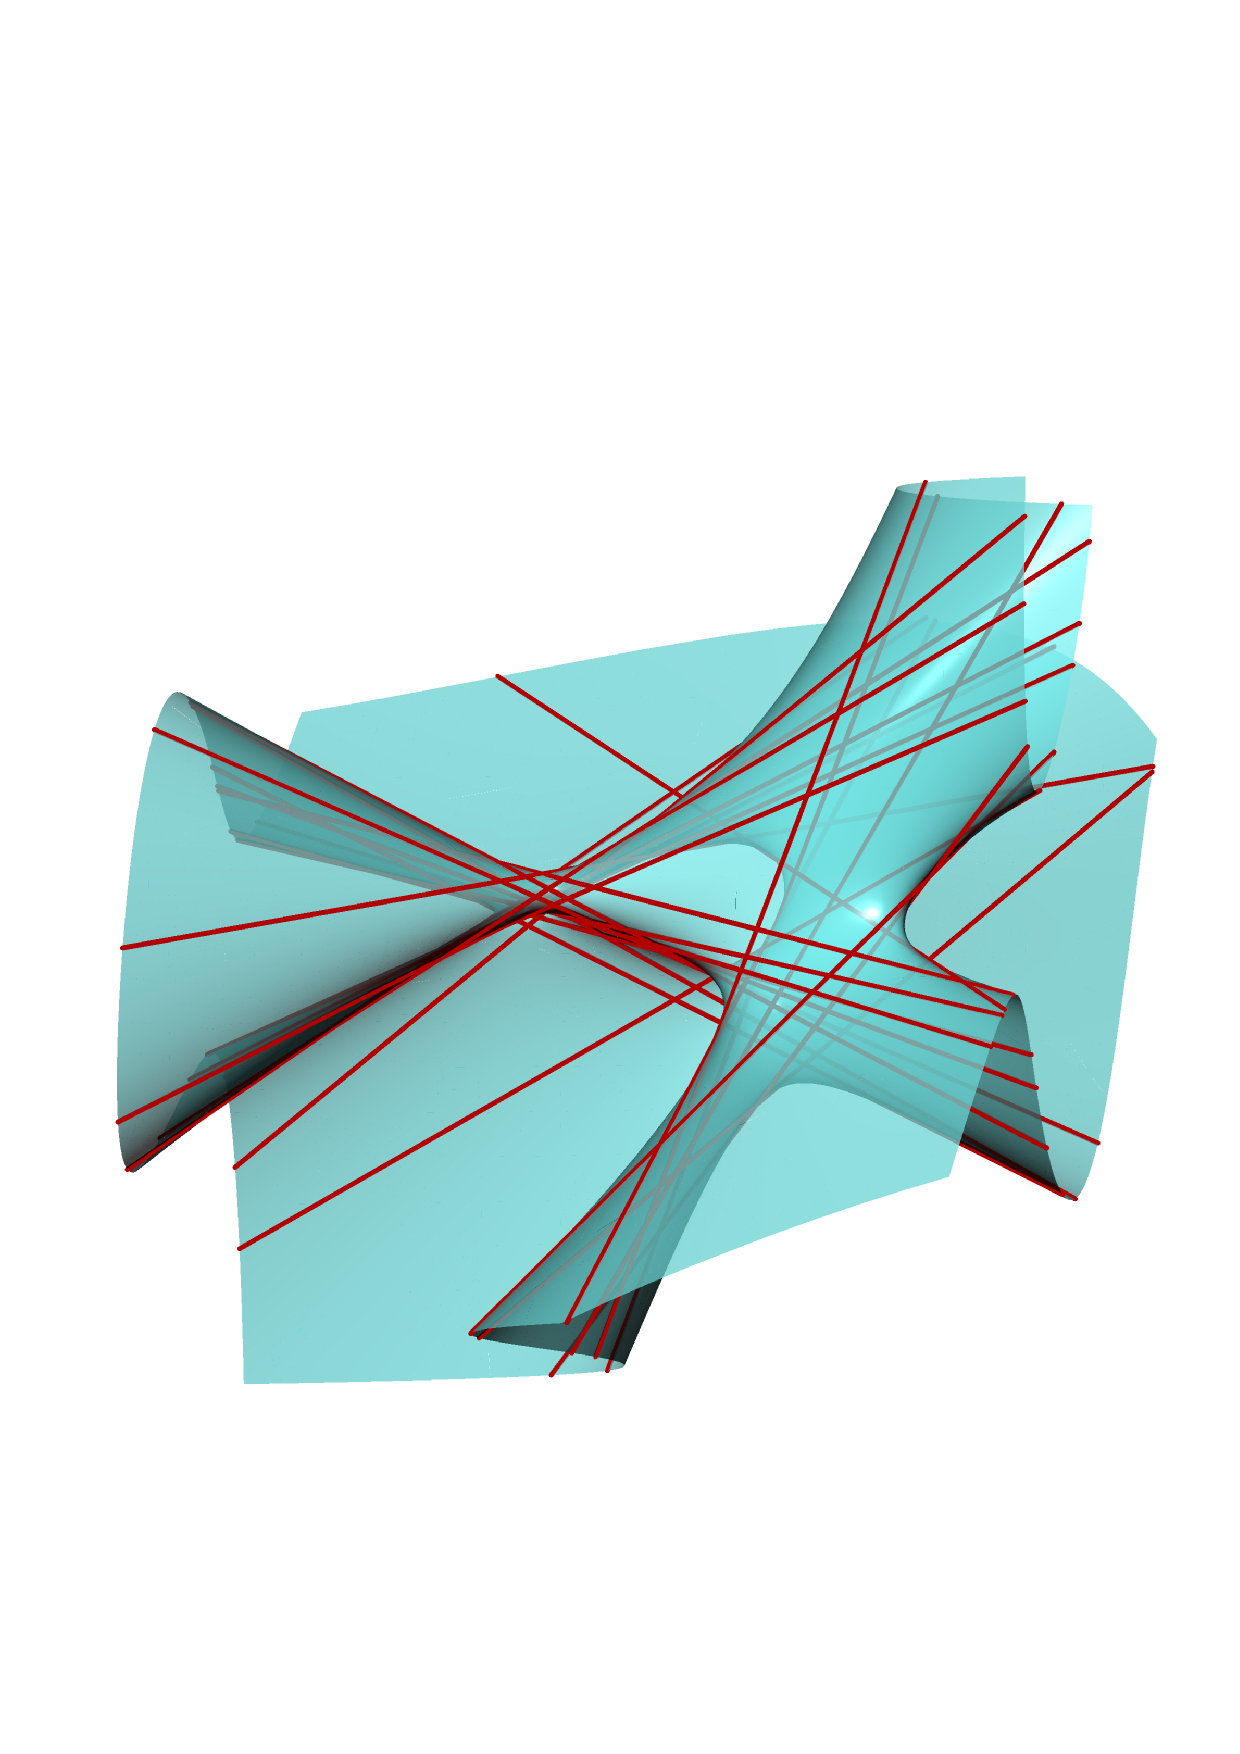
\includegraphics[scale=.55]{figures/27lines.pdf}
\caption{27 lines on a cubic surface}
\end{figure}
\end{center}


\begin{thm}[Debarre/Manivel]
\vspace{.2cm}
The combinatorial data $(r,n,d_\bullet)$ determines a Fano problem when $n-s-2r\ge 0$ and
\begin{align*}
(r+1)(n-r) - \sum_{i=1}^s \begin{pmatrix}d_i + r\\r\end{pmatrix}=0.
\end{align*}
\vspace{.1cm}
\end{thm}
%\begin{enumerate}
%\item[$\bullet$] [Debarre/Manivel] The combinatorial data $(r,n,d_\bullet)$ determines a Fano problem when $n-s-2r\ge 0$ and
%\vspace{-.5cm}
%\hspace{-1.2cm}
%\begin{minipage}{.99\textwidth}
%\begin{align*}
%(r+1)(n-r) - \sum_{i=1}^s \left(\begin{smallmatrix}d_i + r\\r\end{smallmatrix}\right)=0.
%\end{align*}
%\end{minipage}
%\end{enumerate}

%\vspace{.6cm}

%Debarre and Manivel determined the number of solutions to a general Fano problem of type $(r,n,d_\bullet)$, $N(r,n,d_\bullet)$.

\vspace{.8cm}

\begin{figure}
\begin{minipage}{.99\textwidth}
\begin{table}[htb]
  \label{Small Fano}
  \def\arraystretch{1.2}
  \begin{tabular}{||c|c|c|c|c||}
    \hline
    $~r~$ & $~n~$ & $~d_\bullet~$ & $~N(r,n,d_\bullet)~$\\
    \hline\hline
    1 & 4 & $(2,2)$ & 16\\
    \hline
    1 & 3 & $(3)$ & 27\\
    \hline
    2 & 6 & $(2,2)$ & 64\\
    \hline
    3 & 8 & $(2,2)$ & 256\\
    \hline
    1 & 7 & $(2,2,2,2)$ & 512\\
    \hline
    1 & 6 & $(2,2,3)$ & 720\\
    \hline
  \end{tabular}
\end{table}
\end{minipage}
\caption{All Fano problems with $\le 1000$ solutions}
\end{figure}
\end{minipage}
%
\tallminipage
%%%%%COLUMN 2%%%%%
\begin{minipage}[t]{.3\textwidth}
\headft{Galois groups of Fano problems}
Write $\mathbb{C}^{(r,n,d_\bullet)}$ for the parameter space of homogeneous forms $F = (f_1,\dotsc,f_s)$ in $n+1$ variables of degrees $d_\bullet = (d_1,\dotsc,d_s)$. Consider the incidence correspondence.

\vspace{-1cm}

\begin{center}
\begin{tikzpicture}
\node at (0,0) {$\Gamma_{(r,n,d_\bullet)} = \{(F,\ell)\in \mathbb{C}^{(r,n,d_\bullet)}\times\mathbb{G}(r,\mathbb{P}^n):\ell\in V_r(X_F)\}$};
\node at (-9.3,-4.75) {$\mathbb{C}^{(r,n,d_\bullet)}$};
\draw[very thick,->] (-9.3,-1.3)--(-9.3,-4.05) node[left] at (-9.4,-2.875) {$\pi_{(r,n,d_\bullet)}$};
\draw[very thick,->] (-9,-1.3)--(1.5,-4) node at (1.5,-4.75) {$\mathbb{G}(r,\mathbb{P}^n)$};
\end{tikzpicture}
\end{center}

%\vspace{-.45cm}

%\begin{enumerate}
%\item[$\bullet$] $\deg \pi_{(r,n,d_\bullet)} = N(r,n,d_\bullet)$.

%\item[$\bullet$] $\pi_{(r,n,d_\bullet)}$ restricts to a covering space over a Zariski open set.
%\end{enumerate}

\vspace{1cm}

\begin{minipage}{.65\textwidth}
The \blue{Galois group}, $\mathcal{G}_{(r,n,d_\bullet)}$, of the Fano problem determined by $(r,n,d_\bullet)$ is the monodromy group of $\pi_{(r,n,d_\bullet)}$.
\begin{enumerate}
\item[$\bullet$] $\mathcal{G}_{(r,n,d_\bullet)}$ is transitive

\item[$\bullet$] $\mathcal{G}_{(r,n,d_\bullet)}$ is a Galois group in the algebraic sense.
\end{enumerate}
\end{minipage}
%
\begin{minipage}{.02\textwidth}
~
\end{minipage}
%
\begin{minipage}{.3\textwidth}
\begin{center}
\begin{figure}
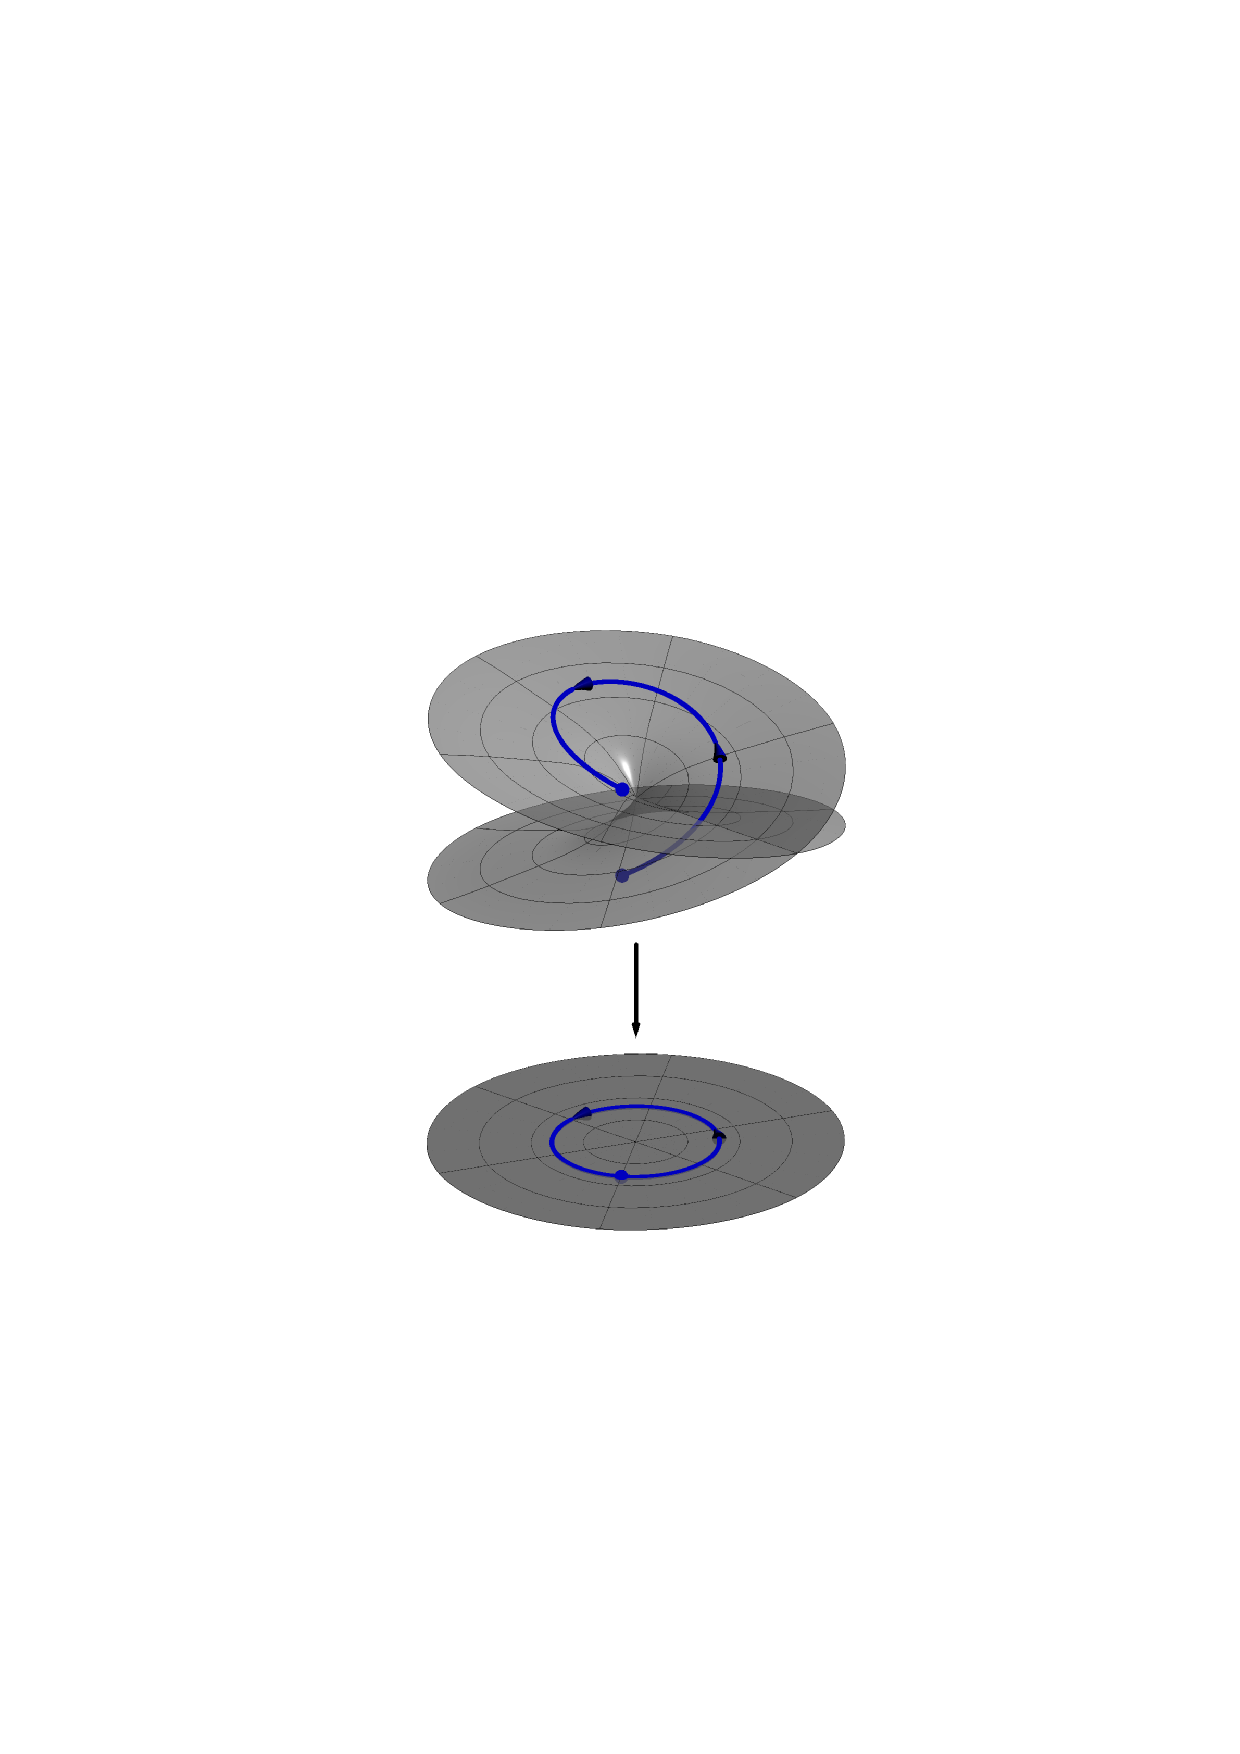
\includegraphics[scale=.95]{figures/monodromy.pdf}
\end{figure}
\end{center}
\end{minipage}

\vspace{.4cm}

\begin{thm}[Jordan,Harris,Hashimoto,Kadets]
\vspace{.2cm}
The following is known:
\begin{enumerate}
\item[$\bullet$] [J],[Har] $\mathcal{G}_{(1,3,(3))} = E_6$.

\vspace{.4cm}

\item[$\bullet$] [Has,K] $\mathcal{G}_{(r,2r+2,(2,2))} = D_{2r+3}$.

\vspace{.4cm}

\item[$\bullet$] [Has,K] All other $\mathcal{G}_{(r,n,d_\bullet)}$ contain the alternating group.
\end{enumerate}
\vspace{.1cm}
\end{thm}

\vspace{0cm}

%The \blue{Galois group}, $\mathcal{G}_{(r,n,d_\bullet)}$, of the Fano problem determined by $(r,n,d_\bullet)$ is the monodromy group of $\pi_{(r,n,d_\bullet)}$.

%\vspace{.5cm}

%\begin{minipage}{.71\textwidth}
%\begin{enumerate}
%\item[$\bullet$] [Jordan],[Harris] $\mathcal{G}_{(1,3,(3))} = E_6$.

%\vspace{.1cm}

%\item[$\bullet$] [Hashimoto/Kadets] $\mathcal{G}_{(r,2r+2,(2,2))} = D_{2r+3}$.

%\vspace{.1cm}

%\item[$\bullet$] [Hashimoto/Kadets] All other $\mathcal{G}_{(r,n,d_\bullet)}$ contain the alternating group.
%\end{enumerate}
%\end{minipage}
%
%\begin{minipage}{.25\textwidth}
%\begin{center}
%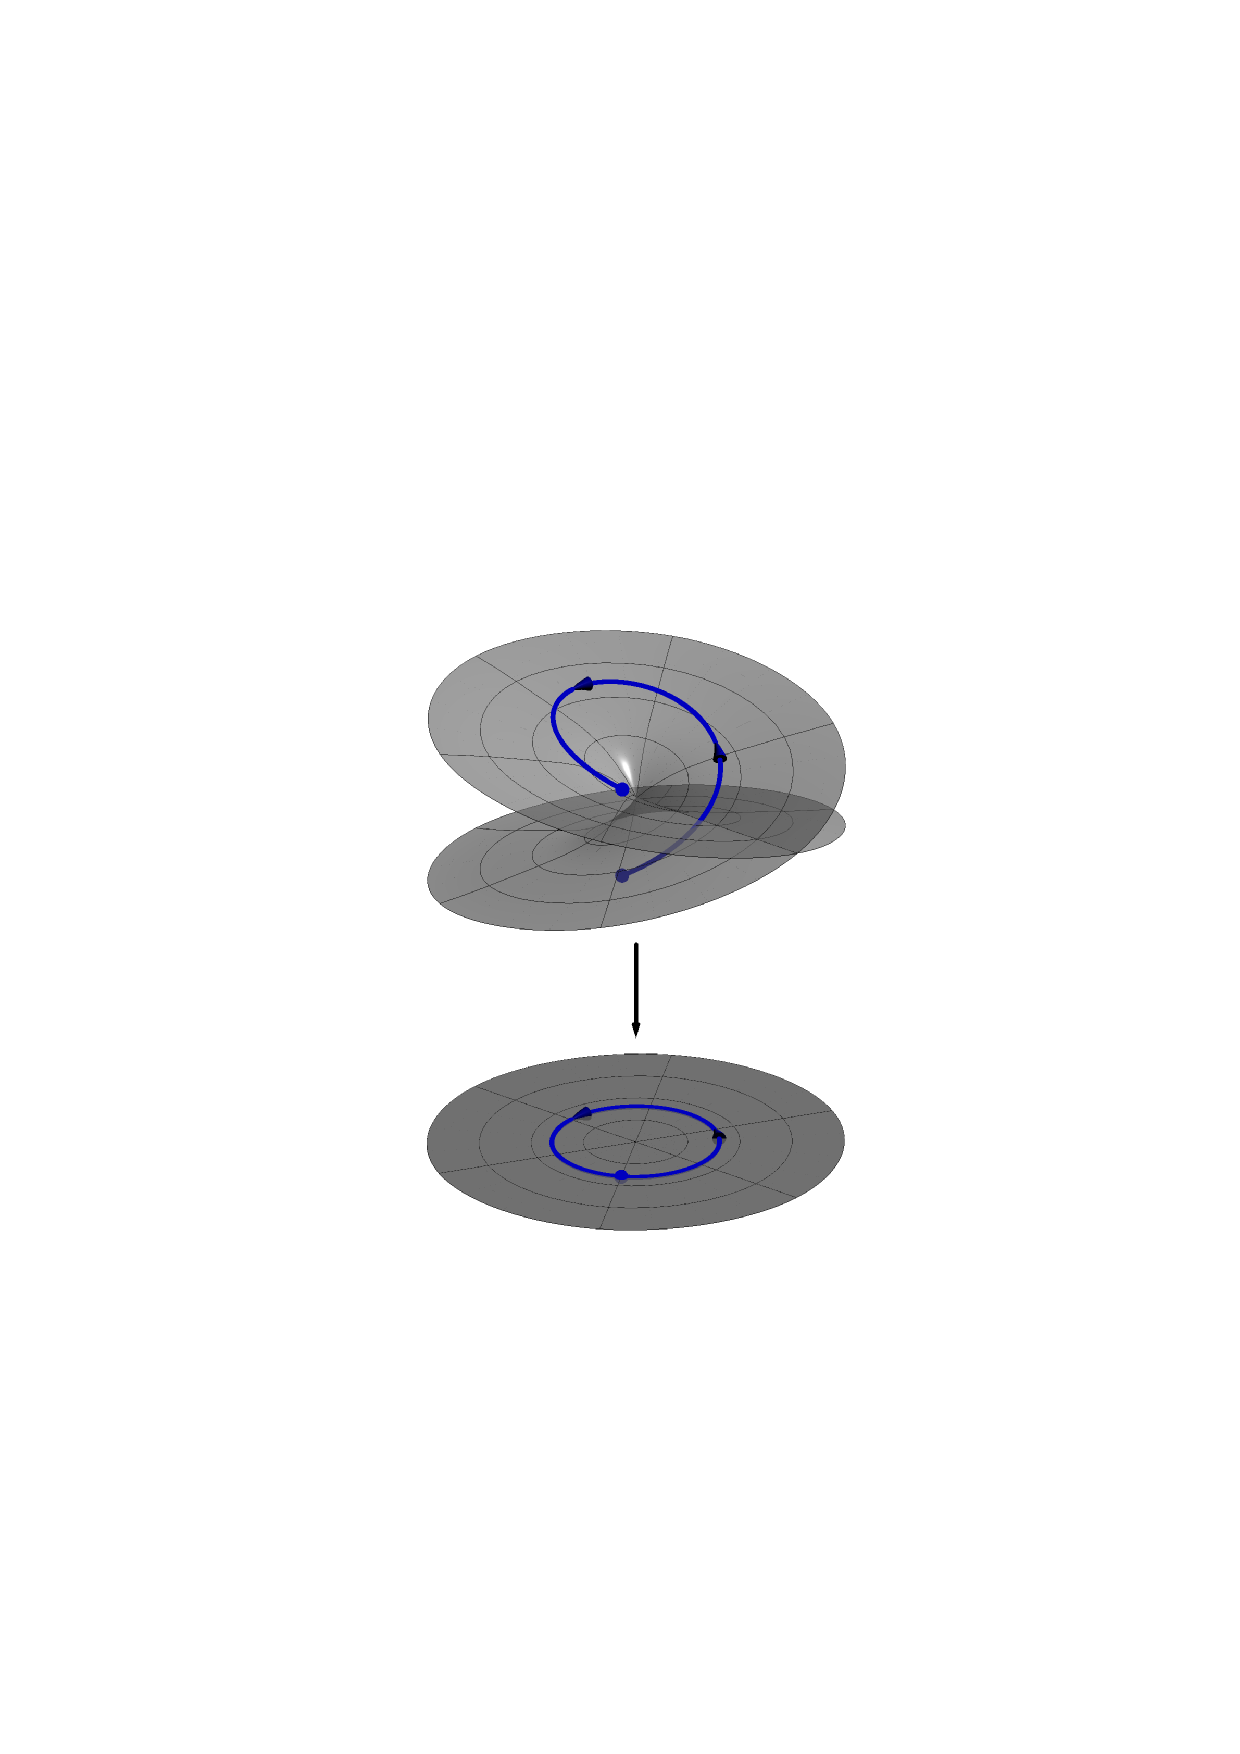
\includegraphics[scale=1]{figures/monodromy.pdf}
%\end{center}
%\end{minipage}

%\vspace{1cm}

\headft{Finding a simple transposition}
\begin{minipage}{.65\textwidth}
Find $F\in\mathbb{C}^{(r,n,d_\bullet)}$ such that $V_r(X_F)$ is one point of multiplicity 2 and $N(r,n,d_\bullet)-2$ smooth points.
\begin{enumerate}
\item[$\bullet$] Heuristically choose $F\in\mathbb{C}^{(r,n,d_\bullet)}$.

\item[$\bullet$] Show $V_r(X_F)$ contains a point of multiplicity 2 by exact computation.

\item[$\bullet$] Show there are $N(r,n,d_\bullet)-2$ smooth points by numerical certification.
\end{enumerate}
\end{minipage}
%
\begin{minipage}{.02\textwidth}
~
\end{minipage}
%
\begin{minipage}{.3\textwidth}
\begin{center}
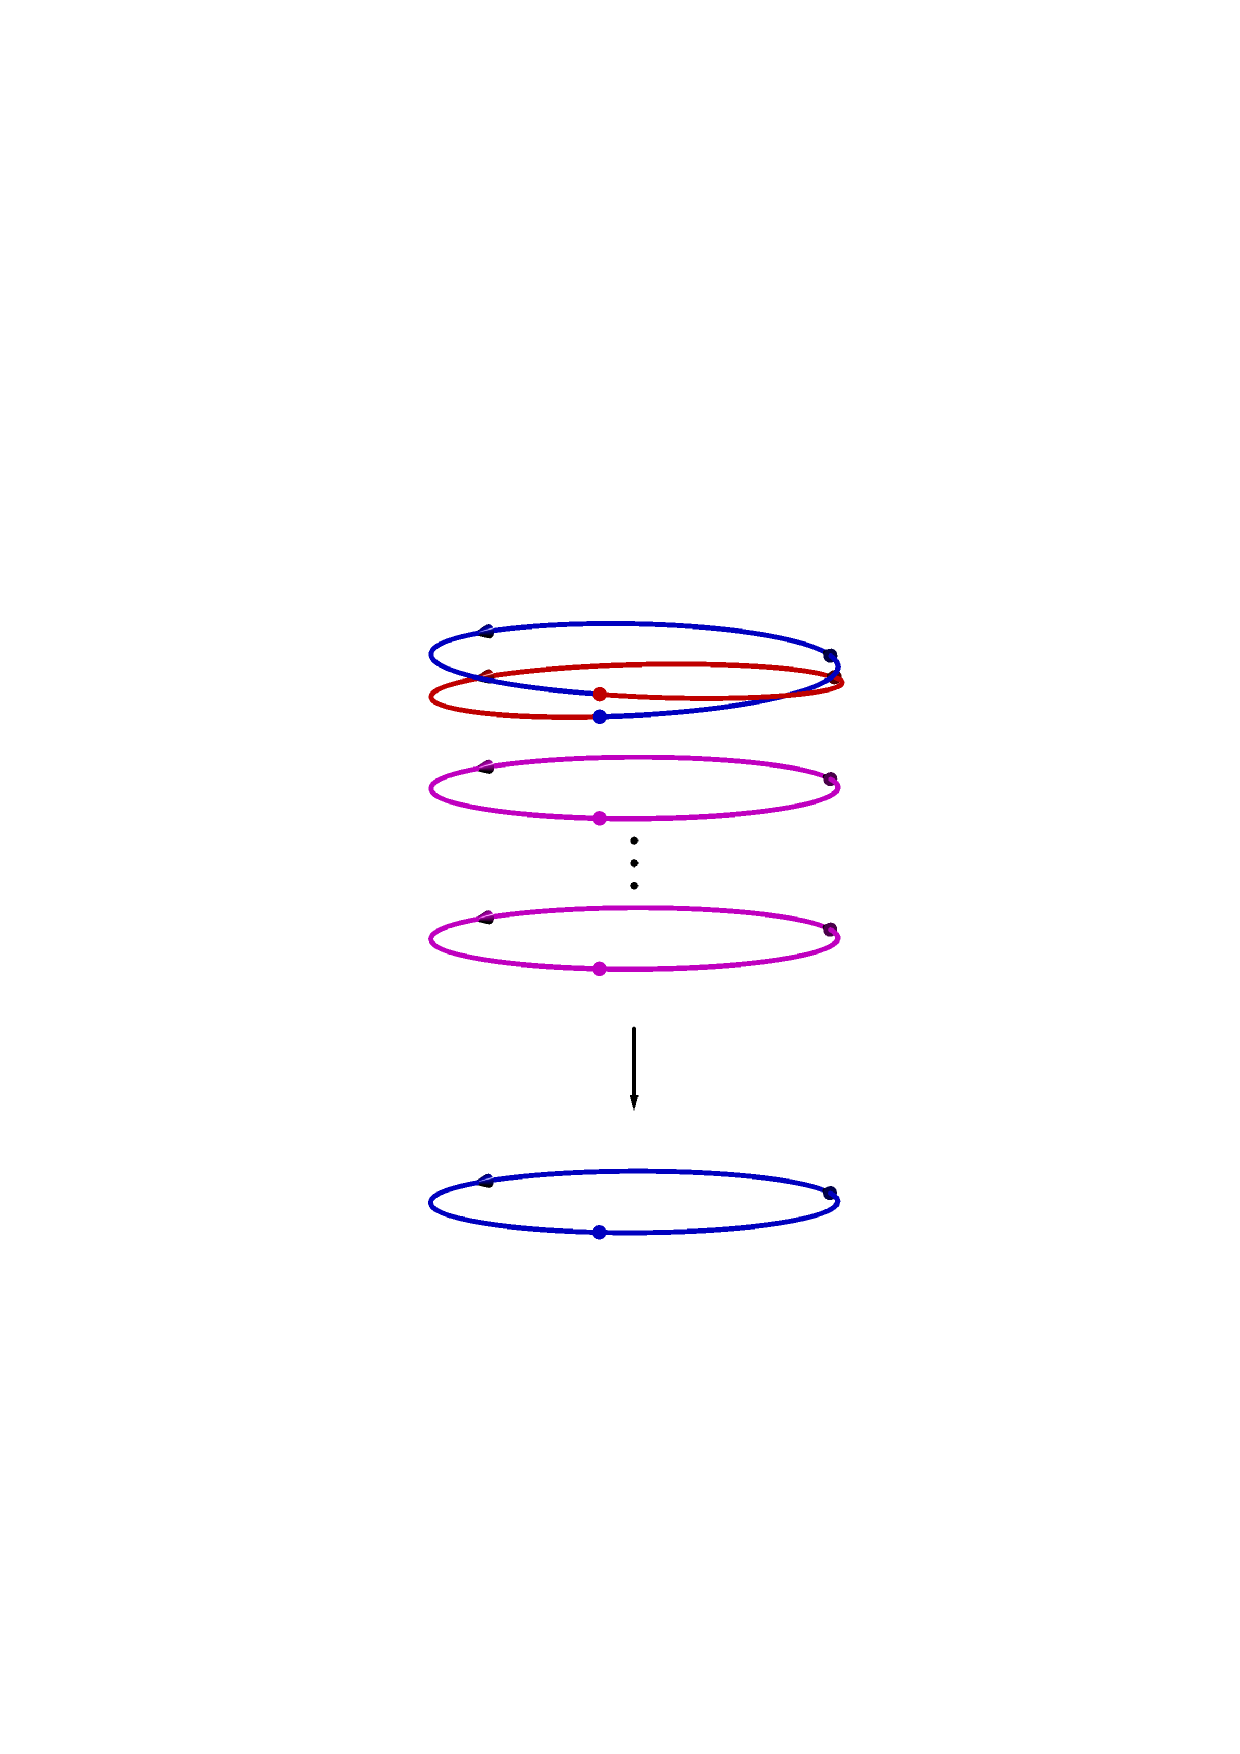
\includegraphics[scale=1]{figures/Harris.pdf}
\end{center}
\end{minipage}

\vspace{1cm}


\end{minipage}
%
\tallminipage
%%%%%COLUMN 3%%%%%
\begin{minipage}[t]{.3\textwidth}
Choose $F$ by presecribing a subscheme of $V_r(X_F)$.
\begin{enumerate}
\item[$\bullet$] Fix an $r$-plane $\ell\in\mathbb{G}(r,\mathbb{P}^n)$ and a tangent vector $v\in T_\ell\mathbb{G}(r,\mathbb{P}^n)$. 

\item[$\bullet$] Choose general $F$ so that $\ell\in V_r(X_F)$ and $v\in T_\ell V_r(X_F)$.
\end{enumerate}

When $\ell$ and $v$ are chosen exactly, $F$ can be chosen exactly as well.
\begin{enumerate}
\item[$\bullet$] [Shub] simple double points are isolated.

\item[$\bullet$] The remaining $N(r,n,d_\bullet)-2$ solutions can be enumerated and isolated by certification.
\begin{enumerate}
\item[\scalebox{.8}{$\blacksquare$}] \Large $\alpha$-theory \normalsize

\item[\scalebox{.7}{$\blacksquare$}] \Large interval arithmetic
\end{enumerate}
\end{enumerate}

\vspace{.1cm}
\headft{Results and timings}
The reported timings for verifying the simple double point and certifying the remaining solutions is given below. (\texttt{alphaCertified},\texttt{HomotopyContinuation.jl})

\vspace{-.8cm}

\hspace{-.2cm}
\begin{minipage}{.99\textwidth}
\begin{table}[htb]
  \label{Big Fano}
  \def\arraystretch{1.2}
  \begin{tabular}{||c|c|c|c|c|c||}
    \hline
    $~r~$ & $~n~$ & $~d_\bullet~$ & $~N(r,n,d_\bullet)~$ & $~\texttt{alCer}$ (h)~ & $~\texttt{HomCo}$ (s)~\\
    \hline\hline
    1 & 7 & $(2,2,2,2)$ & 512 & 2.66 & .61\\
    \hline
    1 & 6 & $(2,2,3)$ & 720  & 2.88 & .87\\
    \hline
    2 & 8 & $(2,2,2)$ & 1024 & 27.32 & 1.57\\
    \hline
    1 & 5 & (3,3) & 1053 & 2.69 & .32\\
    \hline
    1 & 5 & (2,4) & 1280 & 6.09 & .73\\
    \hline
    1 & 10 & (2,2,2,2,2,2) & 20480 & - & 15.44\\
    \hline
    1 & 9 & (2,2,2,2,3) & 27648 & - & 25.97\\
    \hline
    2 & 10 & (2,2,2,2) & 32768 & - & 36.67\\
    \hline
    1 & 8 & (2,2,3,3) & 37584 & - & 38.23\\
    \hline
    1 & 8 & (2,2,2,4) & 47104 & - & 111.88\\
    \hline
  \end{tabular}
\end{table}
\end{minipage}

\vspace{.1cm}

\begin{thm}[Y.]
\vspace{.2cm}
\Large The Fano problems with $d_\bullet\ne (3),(2,2)$ and less than 50,000 solutions have full symmetric Galois group.
\vspace{.1cm}
\end{thm}

Data for these systems and code verifying the data is available at 
\vspace{-.25cm}
\begin{center}
\texttt{github.com/tjyahl/FanoGaloisGroups}
\end{center}
\end{minipage}
%
\tallminipage

\end{frame}
\end{document}



